\documentclass[a4paper]{article}
\usepackage{amsfonts}
\usepackage{amsmath}
\usepackage{amssymb}
\usepackage{graphicx}
\usepackage{float}

\begin{document}
  
\noindent \large Auteur: Siebe Mees \\
\noindent \large Studierichting: Informatica\\
\noindent \large Oefeningenreeks 5G nr. 1.13\\

\medskip

\normalsize

$f(x)=\sqrt{x}\sqrt[4]{1-x} $ op $ \left[0,1\right]$\\

\begin{tabular}{c|ccccc}

$x$ & $0$ & & $\dfrac{2}{3}$ & & $1$ \\ \hline

$f(x)$ & $0$ & & $+$ & & $0$ \\

$f'(x)$ & $+$ & & $0$ & & $-$ \\

$f''(x)$ & $-$ & & $-$ & & $-$ \\ \hline

$f(x)$ & $0$ & $\nearrow$ & $M\left(\dfrac{\sqrt{2}}{3^{\tfrac{3}{4}}}\right)$ & $\searrow$ & $0$ \\

 &  & $\smile$ &  & $\frown$ & \\

\end{tabular}\\

\begin{figure}[H]
\centering
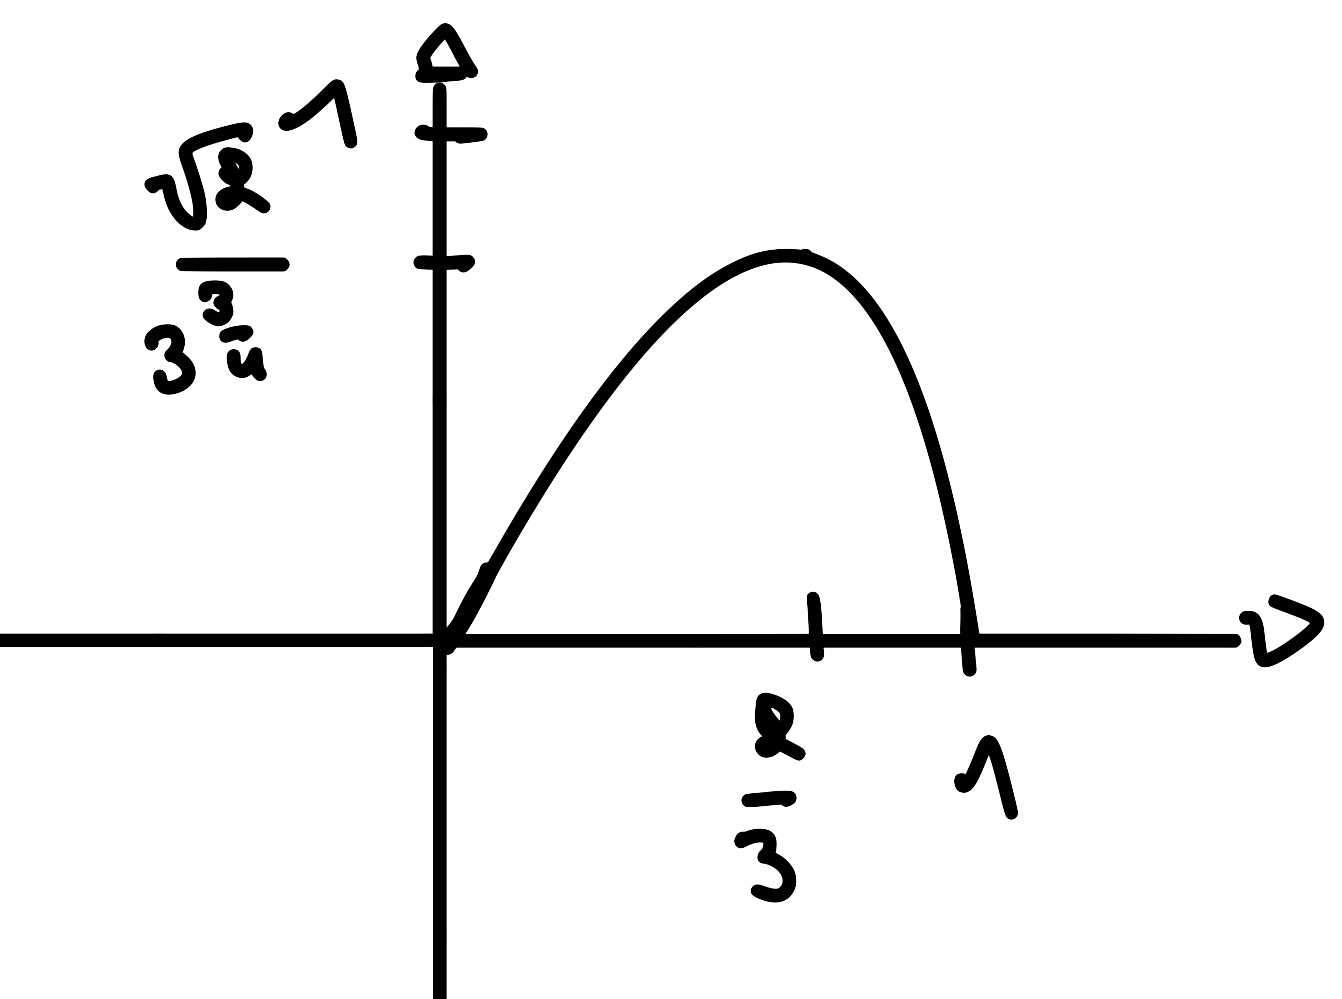
\includegraphics[width=5cm]{5G-1.13-siebe.mees.INF.png}
\end{figure}

$V=\pi \displaystyle\int_0^1 \left(\sqrt{x}\sqrt[4]{1-x}\right)^2 dx$\\

$=\pi \displaystyle\int_0^1 x\sqrt{1-x} dx$\\

$t=1-x \left(x=1-t,\ dx=-dt\right)$\\

$=\pi \displaystyle\int_1^0 (1-t)\sqrt{t}(-dt)$\\

$=\pi \displaystyle\int_0^1 (1-t)t^{1/2} dt$\\

$=\pi \displaystyle\int_0^1 \left(t^{1/2}-t^{3/2}\right) dt$\\

$=\pi \left[\dfrac{2}{3}t^{3/2}-\dfrac{2}{5}t^{5/2}\right]_0^1$\\

$=\pi \left(\dfrac{2}{3}-\dfrac{2}{5}\right)$\\

$=\dfrac{4\pi}{15}$\\

\begin{thebibliography}{999}
%\bibitem{a} Referentie
\end{thebibliography}
\end{document} 
